\documentclass{beamer}
\usetheme{Oxygen}
\usepackage{graphicx}
\usepackage{setspace,cite} % Doble espacio para texto, espacio singular para
                          
\title{\large  M\'etricas de desempe\~no para Maquinas de Aprendizaje}
\author{Juliana Le\'{o}n, Karen Troiano, Stefano De Colli}
\begin{document}
\fontfamily{tahoma}
\frame{\titlepage}

\section*{}
\begin{frame}
  \frametitle{\'{I}ndice}
  \tableofcontents[section=1,hidesubsections]
\end{frame}

\AtBeginSection[]
{
  \frame<handout:0>
  {
    \frametitle{\'{I}ndice}
    \tableofcontents[currentsection,hideallsubsections]
	  }
}

\AtBeginSubsection[]
{
  \frame<handout:0>
  {
    \frametitle{\'{I}ndice}
    \tableofcontents[sectionstyle=show/hide,subsectionstyle=show/shaded/hide]
  }
}

\newcommand<>{\highlighton}[1]{%
  \alt#2{\structure{#1}}{{#1}}
}

\newcommand{\icon}[1]{\pgfimage[height=1em]{#1}}

\section{Introducci\'{o}n}

\begin{frame}
  \frametitle{Introducci\'{o}n}
  \begin{block}{M\'etricas para medir desempe\~no}
  \begin{itemize}
  	\item Introduci\'on al problema
    \item Descripci\'on
  \end{itemize}
  \end{block}

\end{frame}

\section{M\'etodos}
\begin{frame}
  \frametitle{M\'etodos Utilizados}
 % \framesubtitle{}

  \begin{block}{M\'etricas}
	\begin{itemize}
	\item Accuracy
	\item Lift
	\item Presion/Recall
	\begin{itemize}
		\item F1
		\item Coeficiente de correlaci\'on de Matthews
	\end{itemize}
	\item Matriz de Confunsi\'on
	\begin{itemize}
		\item Sensibilidad
		\item Especificidad
	\end{itemize}
	\item ROC - Curva
	\item Coeficiente Silhouette
	\end{itemize}		
	\end{block}
\end{frame}


\begin{frame}
  \frametitle{Accuracy}

  \begin{block}{Descripci\'on}
  \begin{itemize}
  \item Veracidad: Errores Sistem\'aticos
  \item Presi\'on: Errores Random
   
  \end{itemize}
  	
  	\[Accuracy= \dfrac{TP+TN}{TP+FP+FN+TN} \] 
  \end{block}
  \begin{block}{Aplicaciones}
  	Aprendizaje de maquinas donde se cuantan con etiquetas
  	\begin{itemize}
  \item Supervisado
  \item No supervisado
   
  \end{itemize}
  \end{block}
\end{frame}

  	
\begin{frame}
  \frametitle{Lift}

  \begin{block}{Descripci\'on}
  	\begin{itemize}

  	\item Reglas de asociaciones
  	\item Una parte de la data
   
  \end{itemize}
  \end{block}
  \begin{block}{Aplicaciones}

  	\begin{itemize}

  	\item Data Mining
  	\item Marketing
 
  \end{itemize}
  \begin{tabular}{|c|c|c|c|c|c|c|c|}
  \hline 
  Antecedente & A & A & A & B & B & B & A \\ 
  \hline 
  Consecuente & 1 & 0 & 0 & 1 & 0 & 1 & 0 \\ 
  \hline 
  \end{tabular} 
  \end{block}
  
\end{frame}

\begin{frame}
  \frametitle{Presicion/Recall}

  \begin{block}{Descripci\'on}
  	\begin{itemize}

  	\item Presicion: Predicci\'on de la clase positiva 
  	\[PPV= \dfrac{TP}{TP+FP} \] 
  	\item Recall: Predicci\'on de la clase negativa
	\[PPV= \dfrac{TN}{TN+FN} \]   
	
  \end{itemize}
  
  \end{block}
 
\end{frame}


\begin{frame}
  \frametitle{F1 score}
	\begin{block}{Descripci\'on}
	 F1 se puede interpretar como una media ponderada de la precisi\'on y la recuperaci\'on, donde una 			puntuaci\'on de F1 alcanza su mejor valor en 1 y peor puntuación a 0.
	\end{block}
  \begin{block}{Definici\'on}
  	\begin{itemize}
  	\item Presion/Recall
  	\[F1= 2 \dfrac{Presion*Recall}{Presion+Recall} \]   
  	\end{itemize}
  \end{block}
\end{frame}
\begin{frame} 
 \frametitle{Coeficiente de correlaci\'on de Matthews}

  \begin{block}{Descripci\'on}
  \begin{itemize}
  	\item Coeficiente de correlaci\'on entre lo observado y lo que se predijo
  	\item Salida : [ -1, 1] 
	\begin{itemize}
	\item -1 : Predici\'on completamente opuesta
	\item 0: No es mejor que random
	\item 1: Predici\'on Perfecta
\end{itemize}	  	
  \end{itemize}
  \end{block}
\end{frame}


\begin{frame}
  \frametitle{Matriz de Confusi\'on}

  \begin{block}{Descripci\'on}
  	Organizaci\'on de los datos para un an\'alisis practico  
 
  \end{block}
  \includegraphics[scale=0.5]{Picture.png} 
  \end{frame}
  \begin{frame}
\frametitle{Matriz de Confusi\'on}
  
  \begin{block}{M\'etricas obtenidas}
  \begin{itemize}
  	\item Sensibilidad: \[TPR=  \dfrac{TP}{TP+FN} \]   
  	\item Especificidad: \[TNR=  \dfrac{TN}{FP+TN} \]  
  	\item Accuracy
  	\item F1 score
  	\item MCC (Coeficiente de correlaci\'on de Matthews)
	\item Eficiencia: \[eff = \dfrac {Sensibilidad + Especificidad}{2}\]
    \end{itemize}
  
  \end{block}
\end{frame}


\begin{frame}
  \frametitle{ROC}

  \begin{block}{Descripci\'on}
  	\begin{itemize}
  	\item Graficar Sensibilidad x Especificidad
  	\item Datos desbalanceados
  	\item Medicina y Biolog\'ia
  	\end{itemize}
  \end{block}

  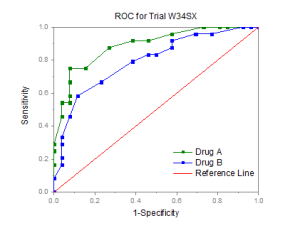
\includegraphics[scale=0.7]{roc.png} 
\end{frame}

\begin{frame}
  \frametitle{Coeficiente de Silhouette}
  \begin{block}{Descripci\'on}
  \begin{itemize}
  \item Es un coeficiente usado para validar Clusters
  	\item Por cada elemento, se calcula el coeficiente de Silhouette para verificar la correctitud de clasificaci\'on
  \end{itemize}
  	
  \end{block}
\end{frame}


\section{Resumen}
\begin{frame}
\frametitle{Resumen}
\begin{block}{}
	\begin{itemize}
	 \item Variedad de m\'etricas
	 \item M\'etricas depende de los datos
	 \item Accuracy no es suficiente
	 \item ROC y Matriz de confusi\'on 
	 \item Sin los datos etiquetados en un problema mas completo \cite{AiRobotics}
	\end{itemize}  
\end{block}

\end{frame}

\begin{frame}

\LARGE{PREGUNTAS}
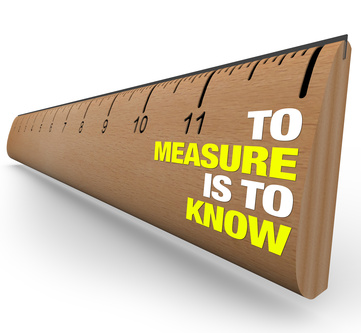
\includegraphics[scale=0.5]{measure.jpg} 
\end{frame}

\begin{frame}[allowframebreaks]
  \frametitle<presentation>{Referencias}    
  \begin{thebibliography}{10}    
   \setbeamertemplate{bibliography item}[online]
  \bibitem{Autor1990}
     HERDIANSYAH HAMZAH.
    \newblock {\em Tools for Machine Learning Performance Evaluation}.
   % \newblock Klein-Verlag, 1990.
  \setbeamertemplate{bibliography item}[online]
  \bibitem{Jemand2000}
   Ron Kohavi
    \newblock Glossary of Terms Special Issue on Applications of Machine Learning and the Knowledge Discovery Process
    \newblock {\em Kluwer Academic Publishers, Boston, Manufactured in The Netherlands}, 1998
    \newblock {http://robotics.stanford.edu/~ronnyk/glossary.html }
  \end{thebibliography}
\end{frame}

\begin{frame}[allowframebreaks]
  \frametitle<presentation>{Referencias}    
  \begin{thebibliography}{10}    
   \setbeamertemplate{bibliography item}[online]
  \bibitem{Autor1990}
  	Wikipedia
    \newblock {\em http://en.wikipedia.org/wiki}.
   
  \end{thebibliography}
\end{frame}

\bibliographystyle{alpha.bst}
\bibliography{referencias}
\end{document}
